\chapter{Букет за мама}

Крайната цел на този проект е децата да създадат букет за своите майки. Когато играчът кликне на това място ще се появи прекрасно цвете. За да се получи най- красивият букет играчът може да променя вида на цветята с помощта на стрелка нагоре. С помощта на лявата и дясната стрелка се променя размерът на цветето.

\begin{figure}[H]
  \centering
  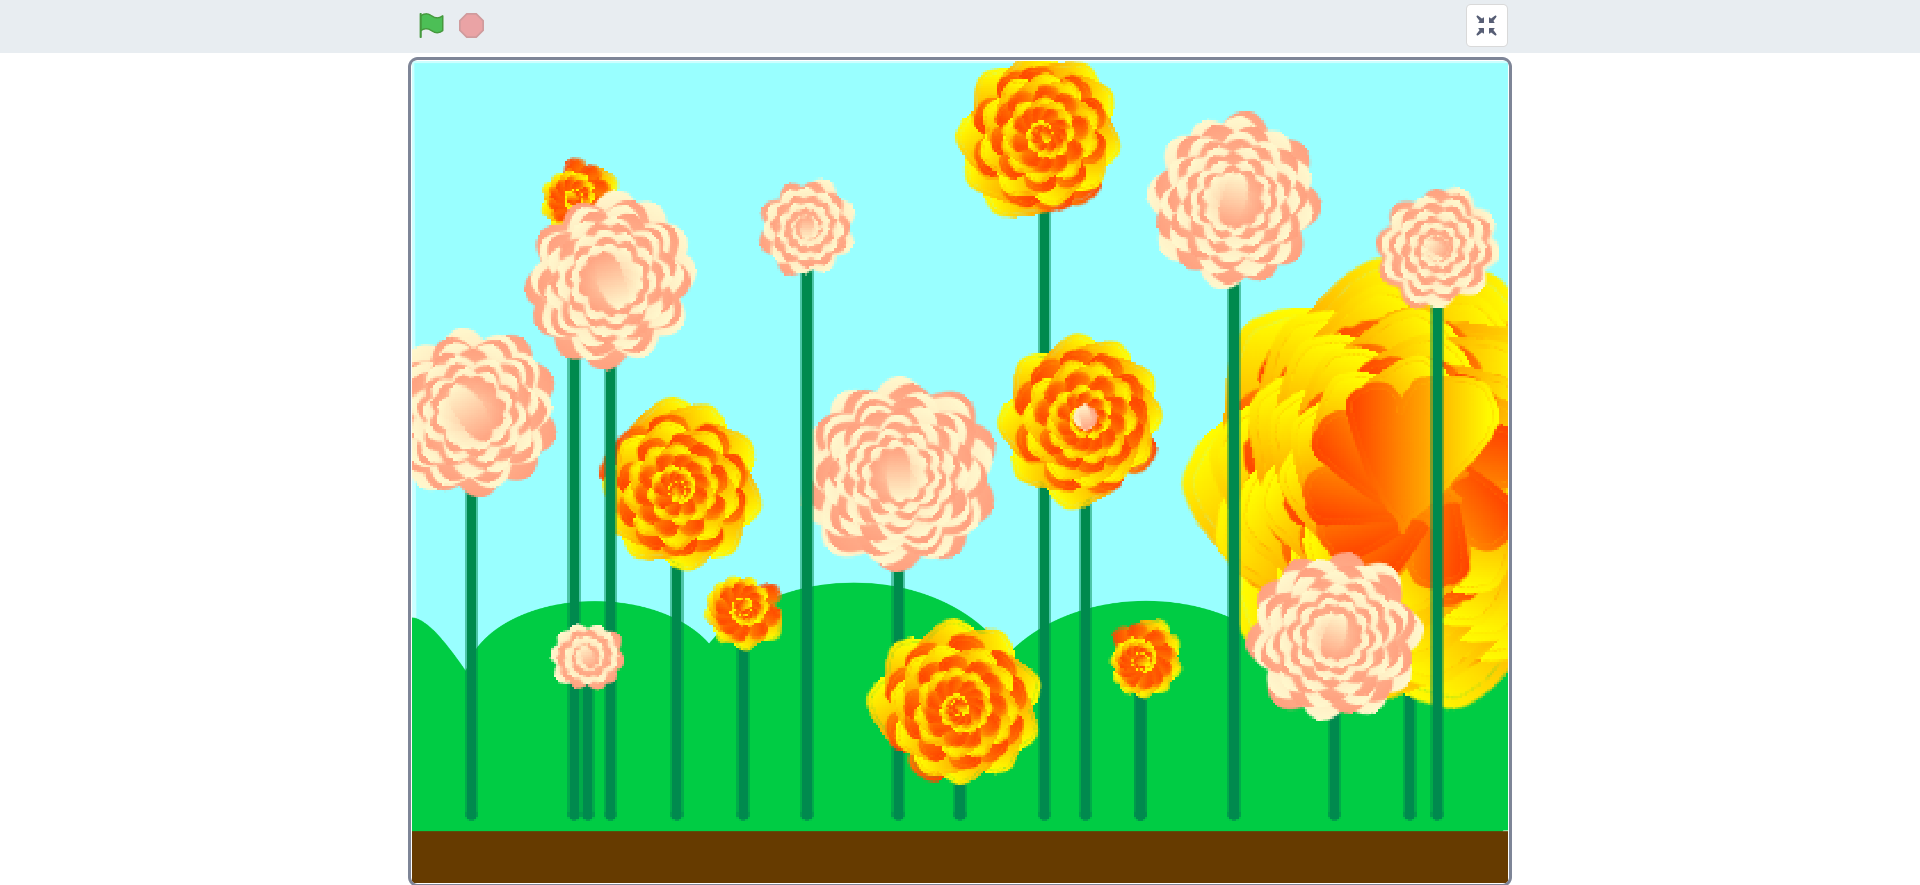
\includegraphics[width=1.0\linewidth,height=0.5\linewidth]{fig040001.png}
  \caption{Букет за мама}
\label{fig040001}
\end{figure}

\section{Добавяне на фон и герои}
Първата стъпка от създаването на играта е добавяне на подходящ фон. От секция Backdrops->Choose a Backdrop може да се избере подходящ от наличните, които Scratch предоставя.

В тази игра няма да има нужда от основния герой в Scratch котката, за това трябва да бъде изтрит.

\begin{figure}[H]
  \centering
  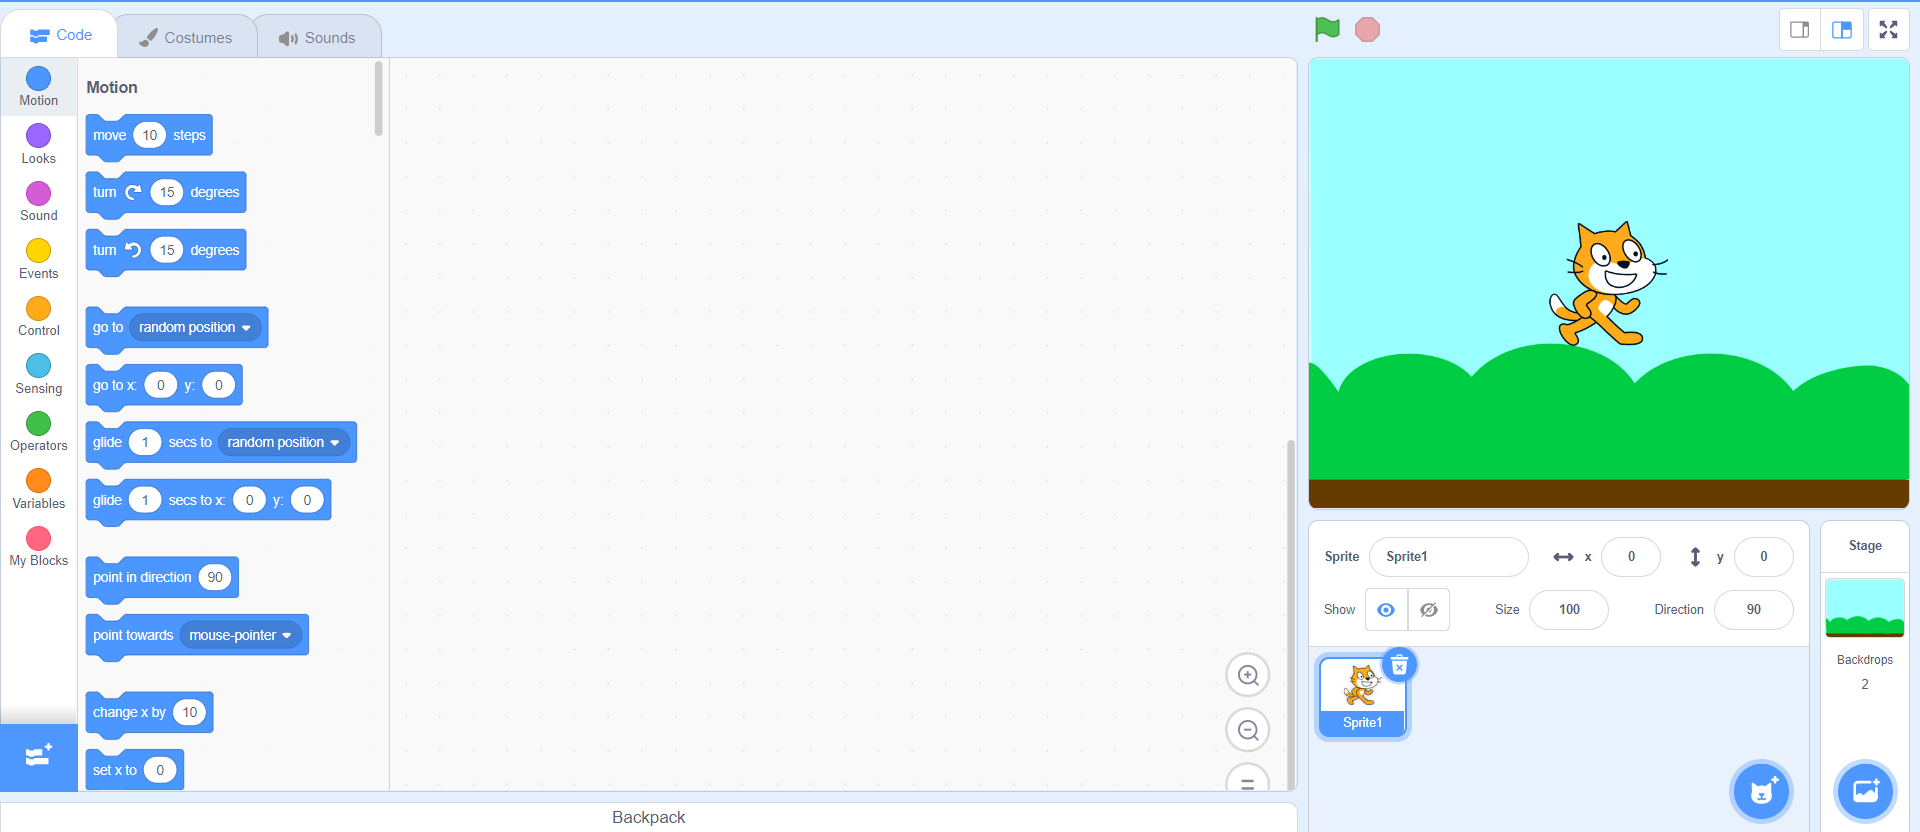
\includegraphics[width=1.0\linewidth,height=0.5\linewidth]{fig040002.png}
  \caption{Фон на играта}
\label{fig040002}
\end{figure}

Следва да се добави героят, който представлява венчелистче на цветето, което ще се създаде, когато играчът кликне върху екранът. Този спрайт трябва да бъде нарисуван използвайки инструментите. За да бъде по- интересна играта може да бъдат добавени повече от един костюм за този герой. Всеки един от костюмите ще представлява различно венчелистче.

\begin{figure}[H]
  \centering
  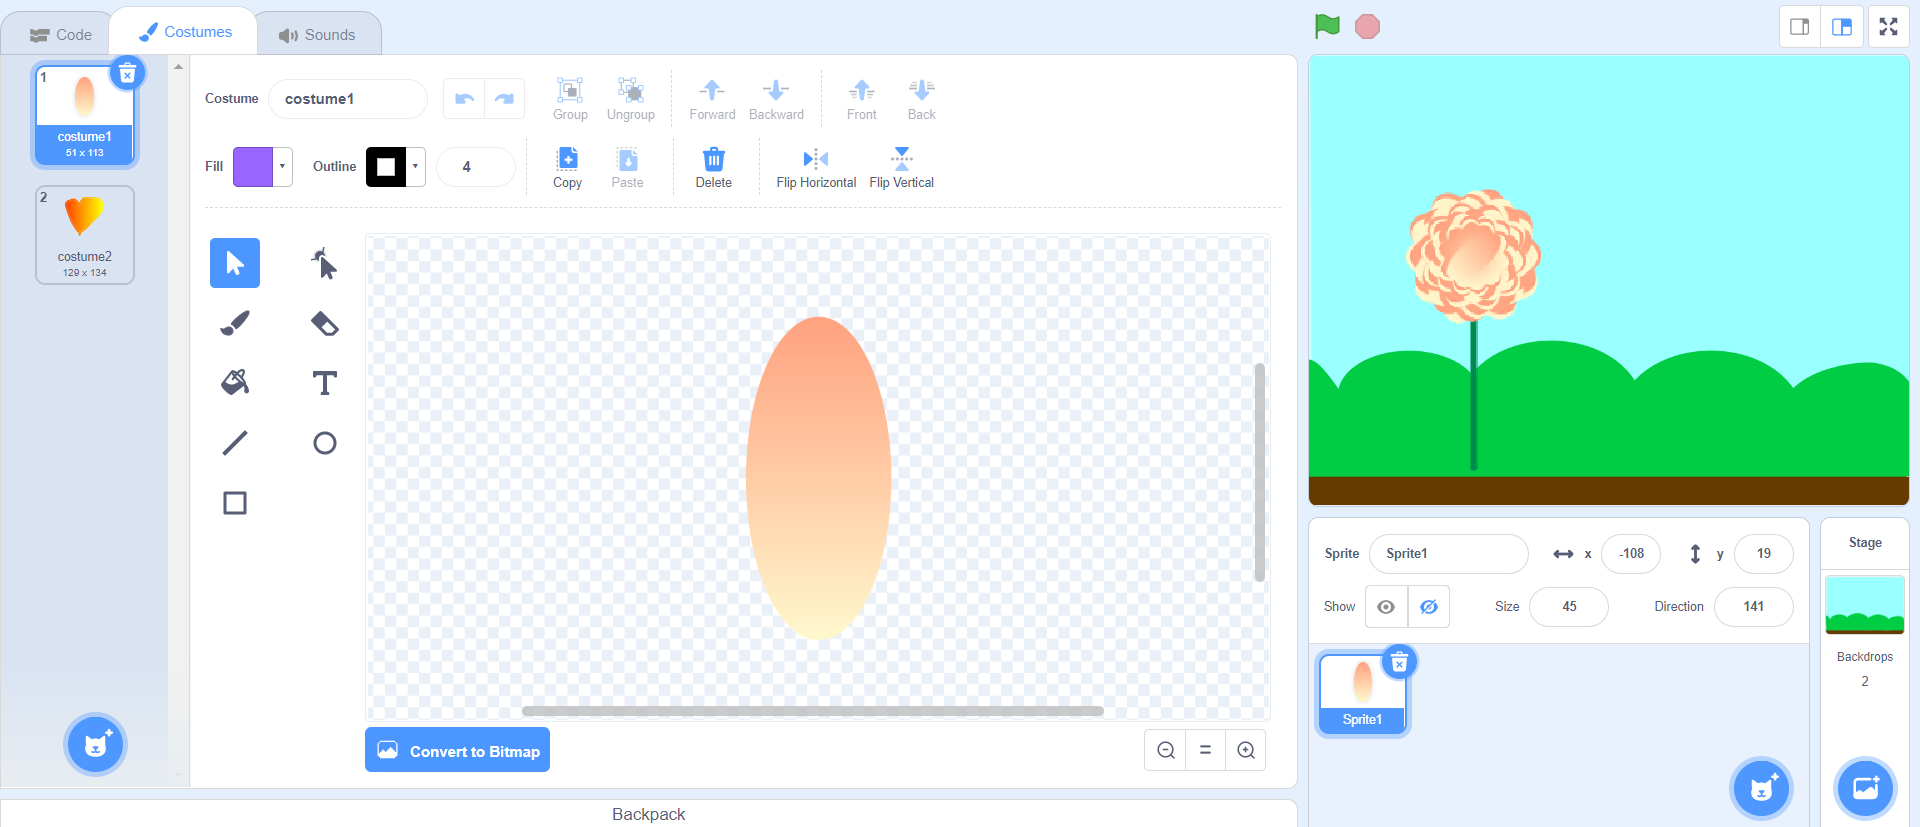
\includegraphics[width=1.0\linewidth,height=0.5\linewidth]{fig040003.png}
  \caption{Рисуване на героя венчелистче}
\label{fig040003}
\end{figure}

\section{Рисуване на цветя}

Когато играчът кликне върху фона ще започне да се рисува цвете. Това означава, че трябва да бъдат поставени инструкции на фона, когато се кликне върху него да изпраща съобщение "draw".

\begin{figure}[H]
  \centering
  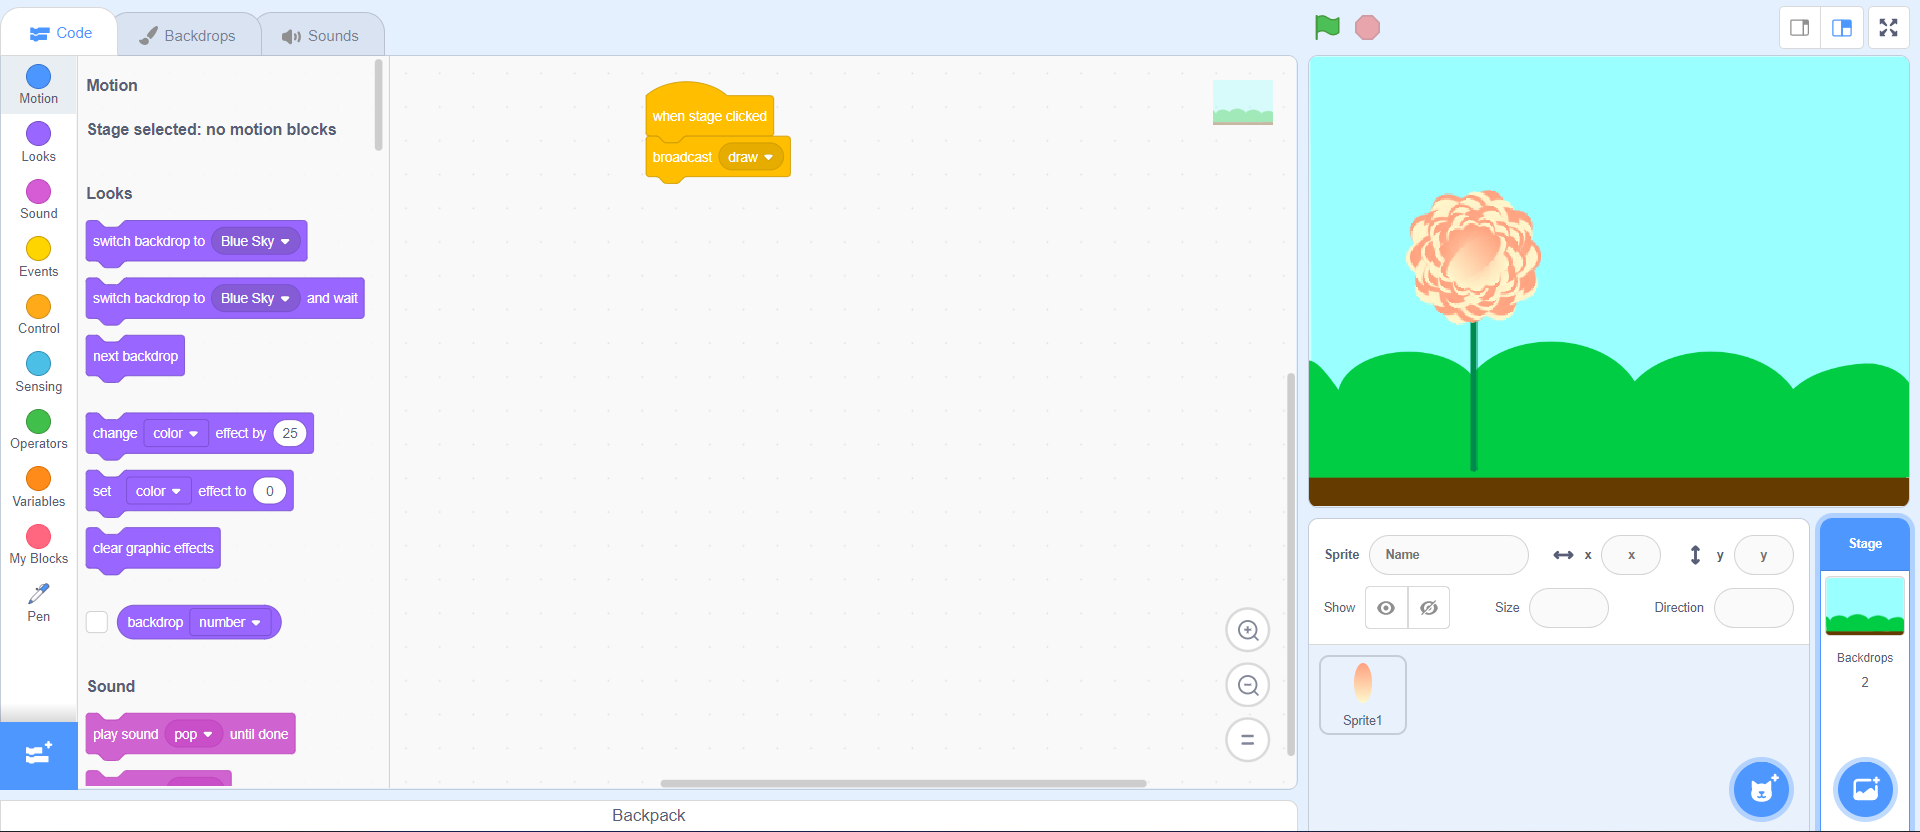
\includegraphics[width=1.0\linewidth,height=0.5\linewidth]{fig040004.png}
  \caption{Инструкции на фона}
\label{fig040004}
\end{figure}

За да се рисуват цветята и стъблата трябва да бъде добавена нова секция с инструкции. Това е секцията Pen.

\begin{figure}[H]
  \centering
  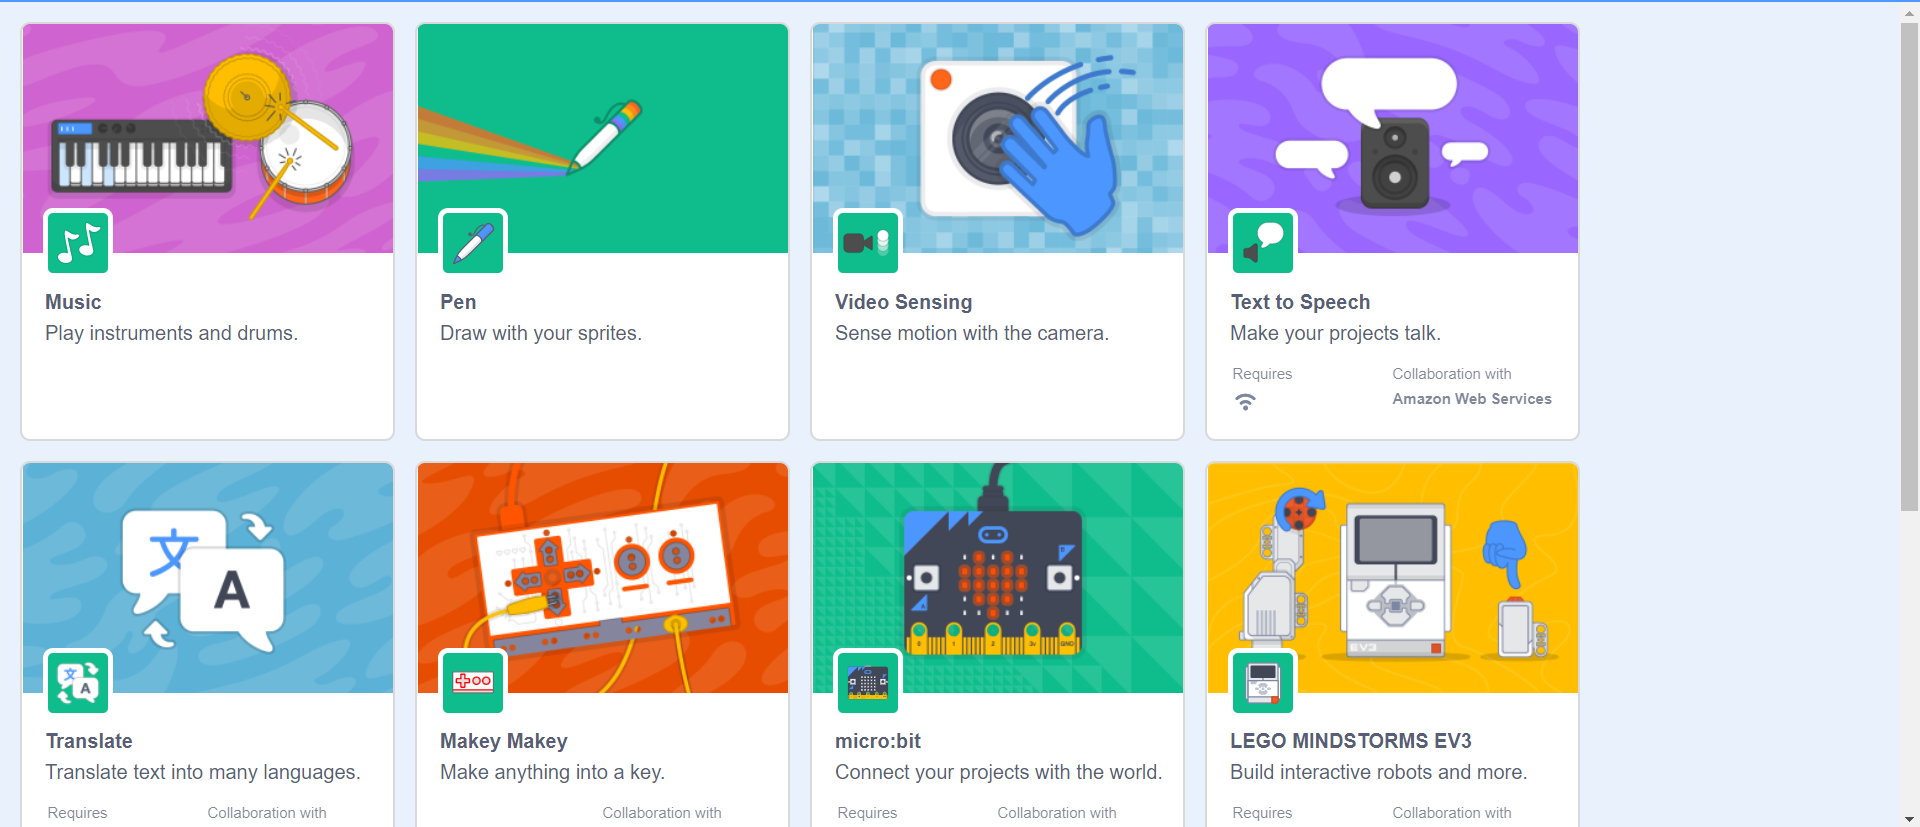
\includegraphics[width=1.0\linewidth,height=0.5\linewidth]{fig040005.png}
  \caption{Добавяне на секция Pen}
\label{fig040005}
\end{figure}

Когато играта започне героят венчелистче трябва да се скрие и всичко нарисувано до този момент да бъде изтрито. Инструкцията, която трие всичко по екрана се намира в новата секция Pen и е "erase all", което означава "изтрий всичко".

\begin{figure}[H]
  \centering
  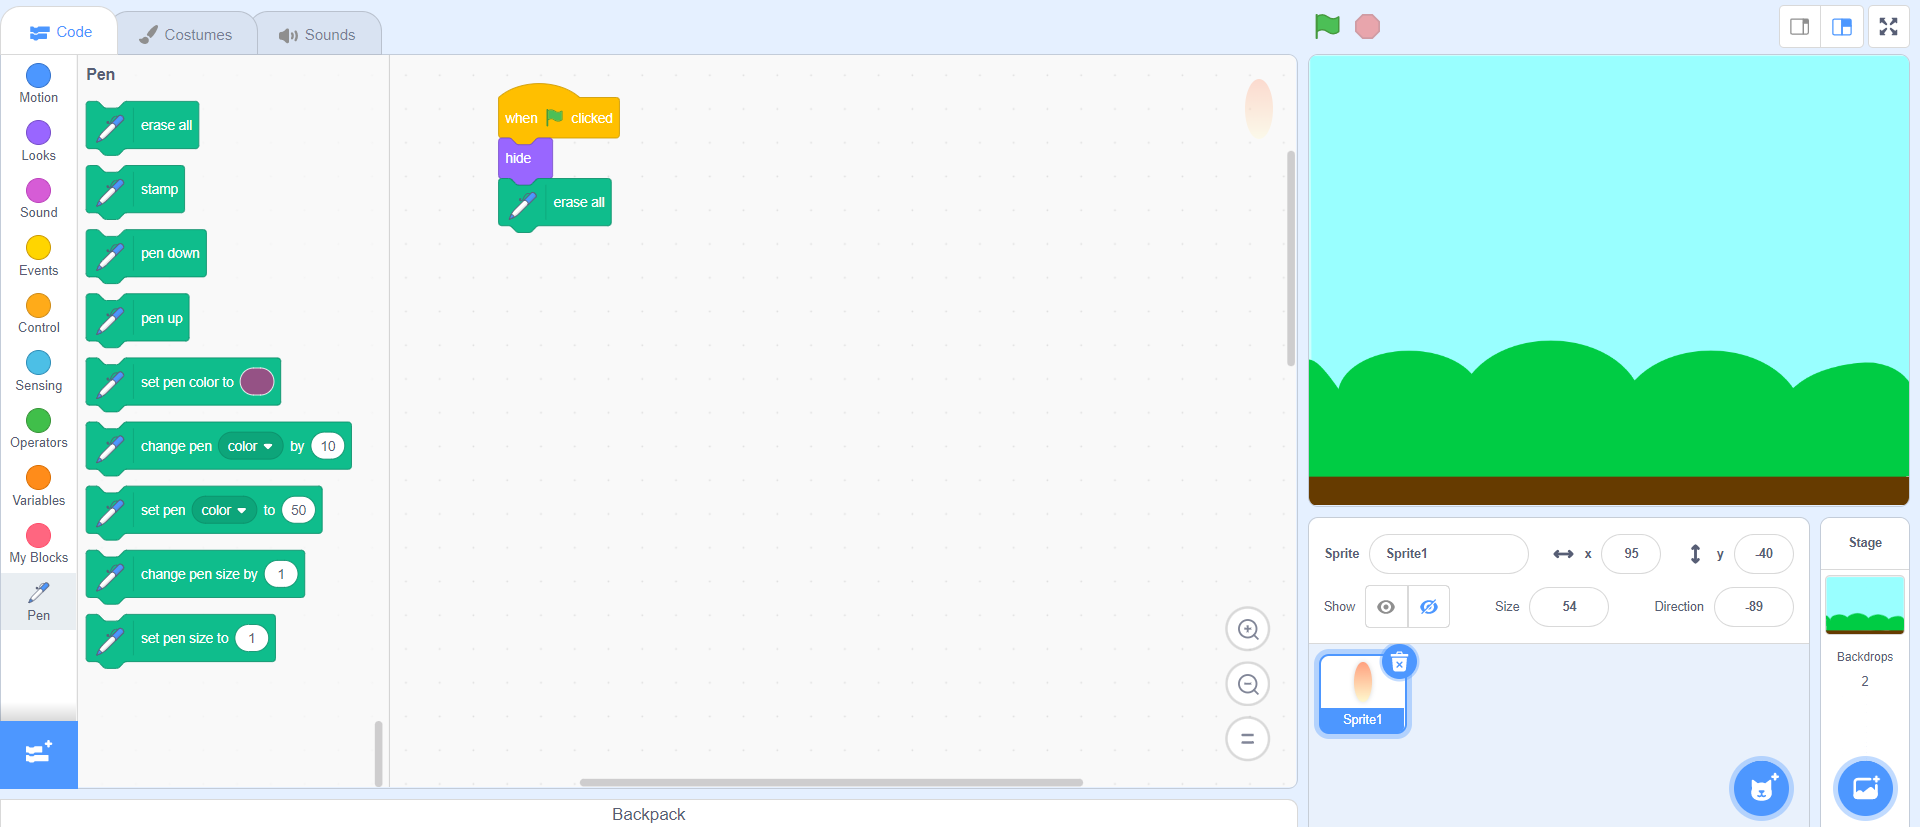
\includegraphics[width=1.0\linewidth,height=0.5\linewidth]{fig040006.png}
  \caption{Начало на играта}
\label{fig040006}
\end{figure}

Преди да се нарисува самото цвете първо ще се нарисува дружката му. Рисуването на дръжката ще започне когато се получи съобщението "draw". Първо ще се зададе дебелина на молива, който ще рисува, както и цветът. Първо трябва да се позиционира моливът. Първоначалната координатата x е същата каквато е тази на мишката в този момент. В светло синята група се намира инструкцията, която дава позицията на мишката за x. Първоначалната координата за y трябва да бъде -150. След като героят е позициониран трябва да се даде инструкция молива да слезе надолу, за да започне да рисува. За да се завърше дръжката на цветето героят трябва да отиде там, където е мишката и да се вдигне молива.

Резултатът от следния код (Фиг. \ref{fig040007}) е, че когато играчът клика върху различни места по екрана ще се нарисуват стъблата на цветята.

\begin{figure}[H]
  \centering
  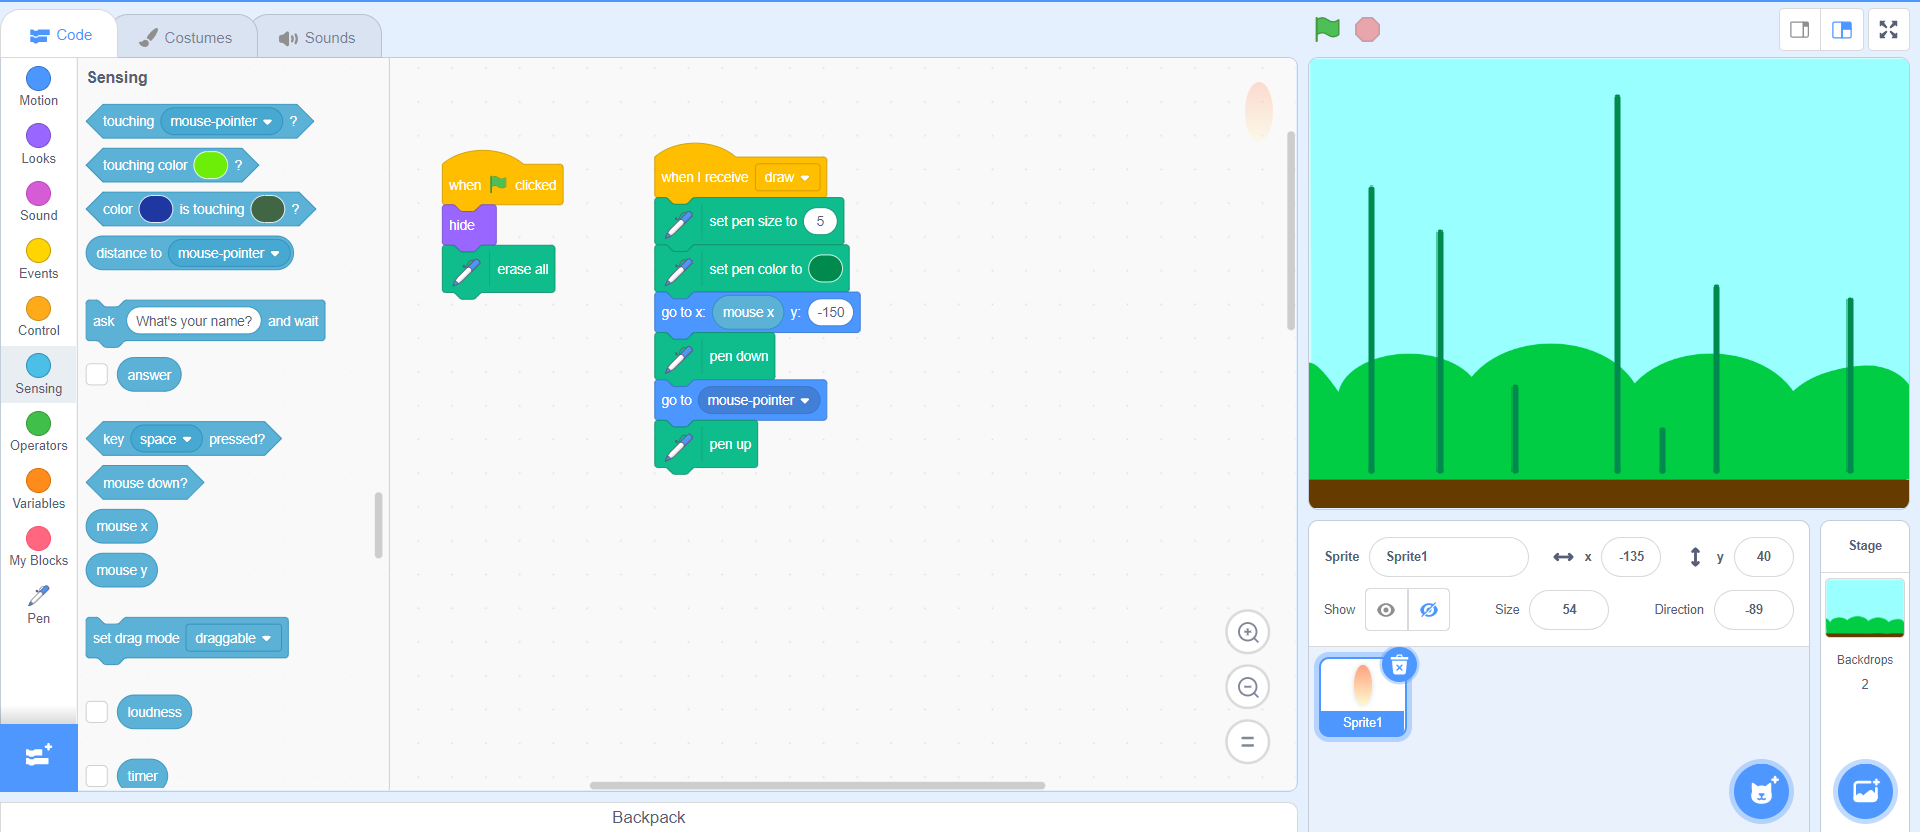
\includegraphics[width=1.0\linewidth,height=0.5\linewidth]{fig040007.png}
  \caption{Рисуване на стеблата на цветята}
\label{fig040007}
\end{figure}

За да се получи цветето трябва героят, който е нарисува да оставя следи, като печат. Всеки път щом остави следа трябва да се завърти и да намали размерът си с едно. Този алгоритъм трябва да се повтори. По този начин се постига ефектът на цветята. За да се получат различни цветя повторенията на алгоритъма за рисуване ще бъде случайно число между 40 и 60.

\begin{figure}[H]
  \centering
  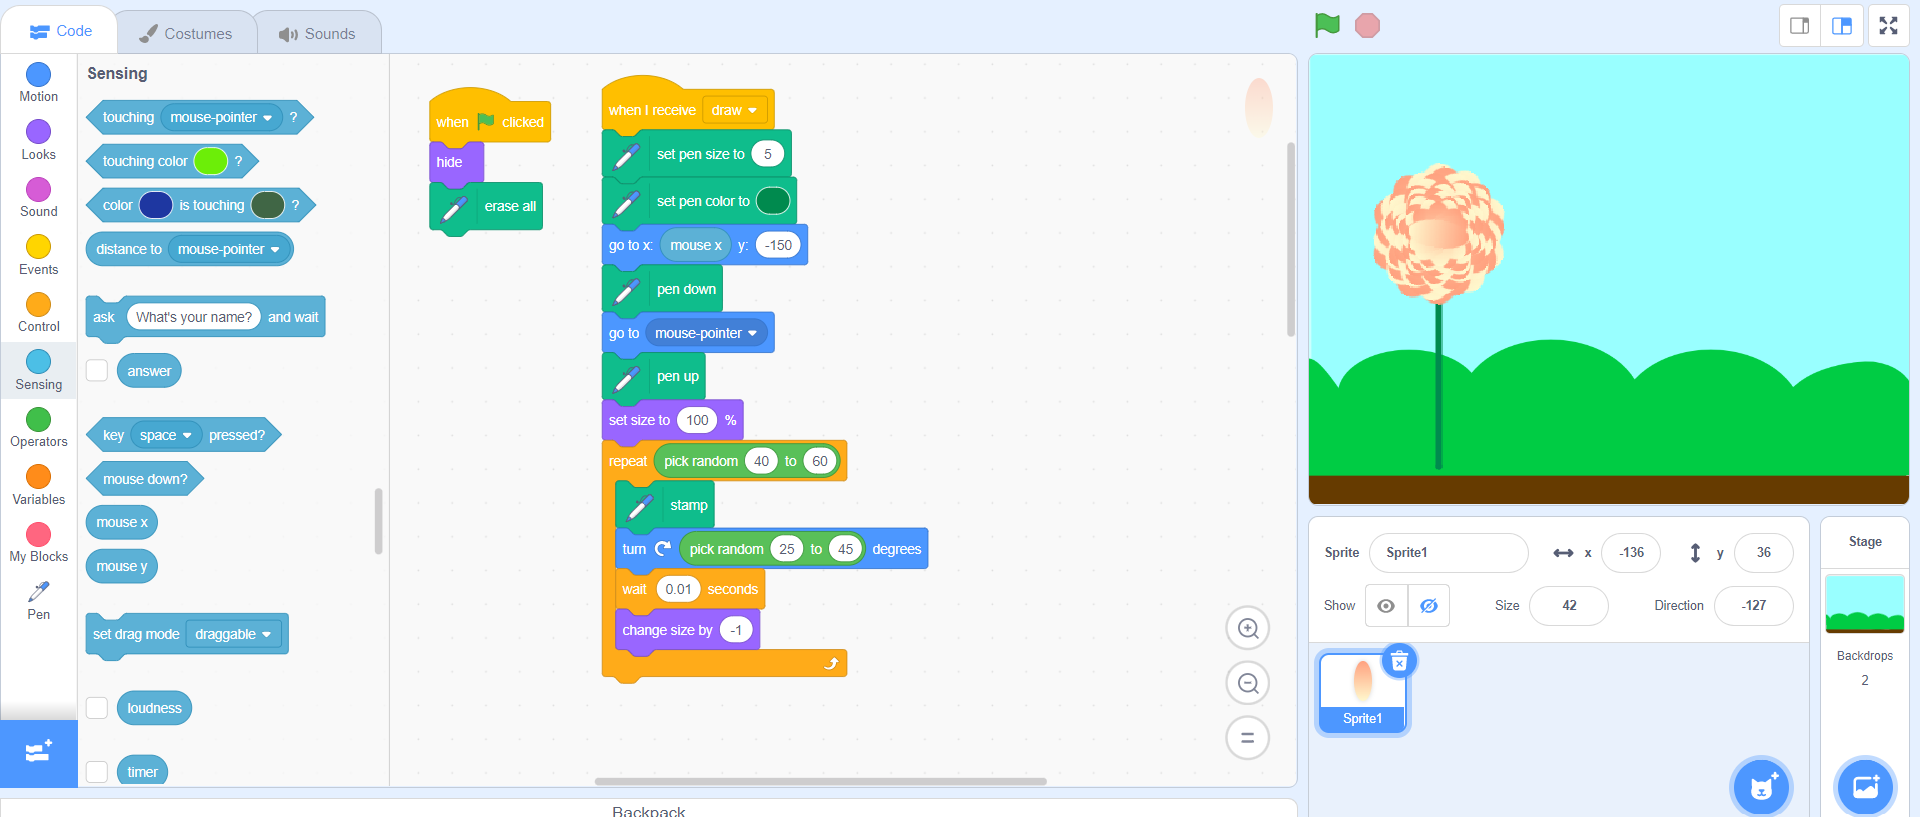
\includegraphics[width=1.0\linewidth,height=0.5\linewidth]{fig040008.png}
  \caption{Рисуване на цветята}
\label{fig040008}
\end{figure}

Резултатът до този момент е, че когато играчът клика върху различни места на екрана ще се появяват цветята за мама.

\section{Промяна на вида и размерите на цветята}

За да се направи по- интересна играта с помощта на стрелка нагоре ще се сменят костюмите на героя. Така колкото повече костюми има, т.е. колкото повече венчелистчета има, толкова по- разнообразен ще бъде букетът.

\begin{figure}[H]
  \centering
  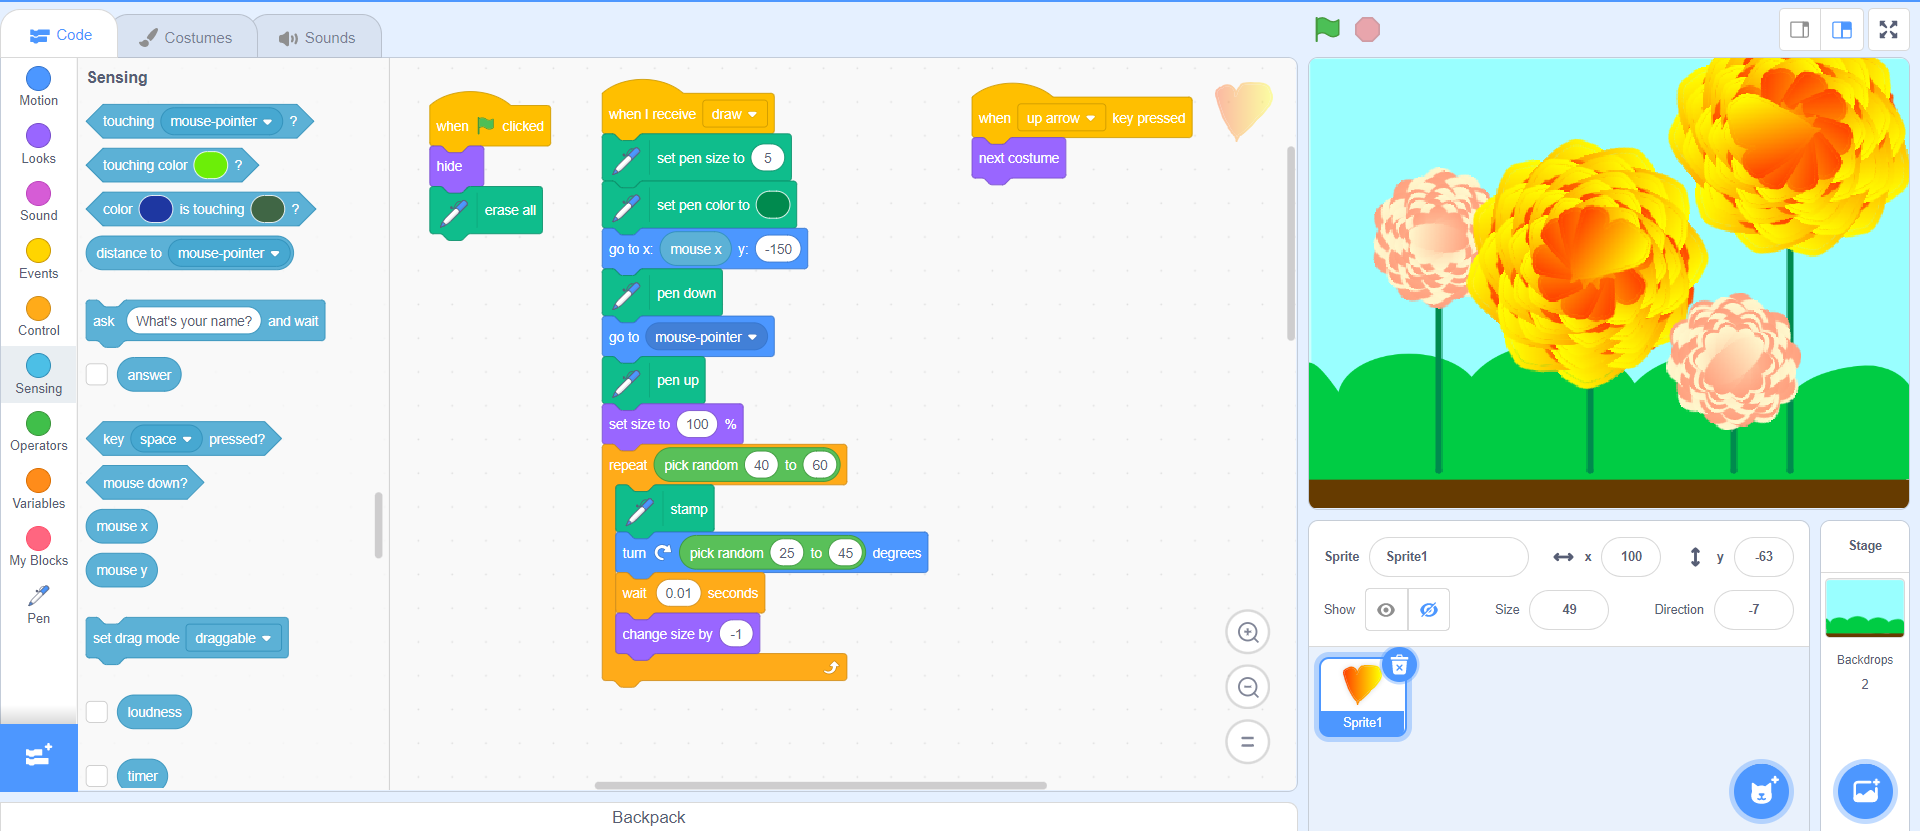
\includegraphics[width=1.0\linewidth,height=0.5\linewidth]{fig040009.png}
  \caption{Променя на костюма на героя}
\label{fig040009}
\end{figure}

Друго подобрение, което може да се направи е да се променя размерът на цветята. За тази цел първото нещо, което трябва да се направи е променлива, която да държи размерът на героя. Характерно за променливите е, че имат първоначална стойност и може да бъде променена тази стойност. В случая първоначалната стойност на променливата ще бъде 100. С натискането на стрелка наляво променливата ще намалява с 10, а при натискане на стрелка надясно - ще се увеличава с 10. Така изглежда финалния код на програмата:

\begin{figure}[H]
  \centering
  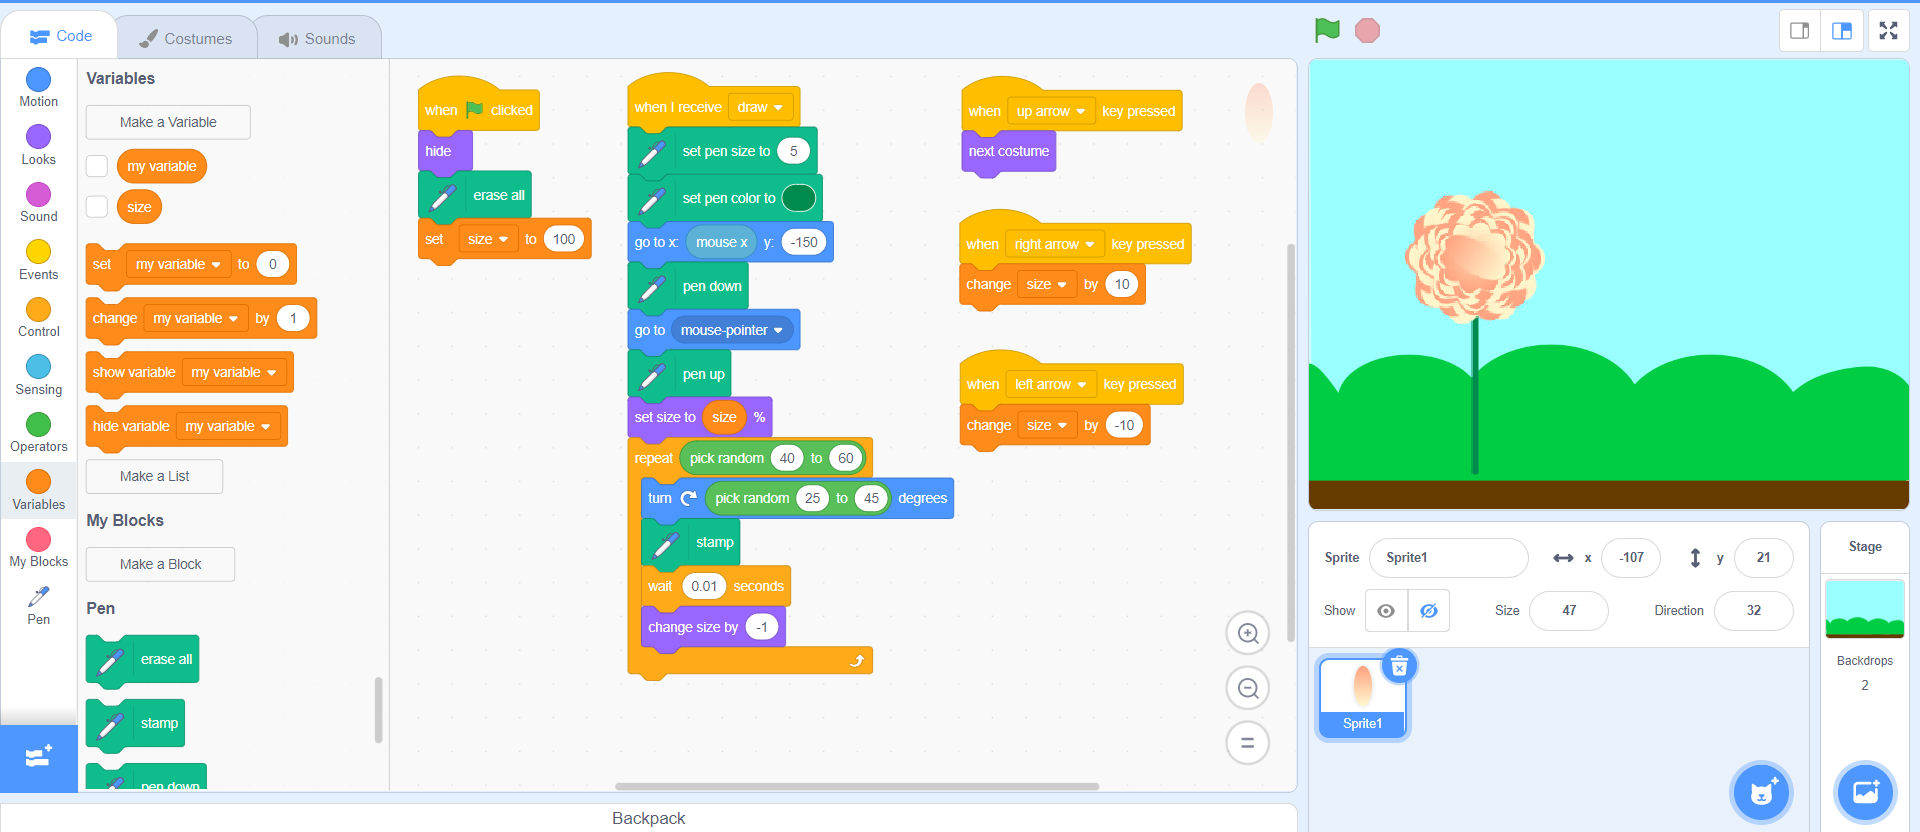
\includegraphics[width=1.0\linewidth,height=0.5\linewidth]{fig040010.png}
  \caption{Целия код на програмата}
\label{fig040010}
\end{figure}

Следва децата да подарят най- красивия букет на своите майки!